% Generated by LitigCharts.PublicationFigures. Captions and provenance are sidecars.
\documentclass[10pt,tikz,border=5pt]{standalone}
\usepackage{lmodern}
\usetikzlibrary{patterns,patterns.meta}
\begin{document}
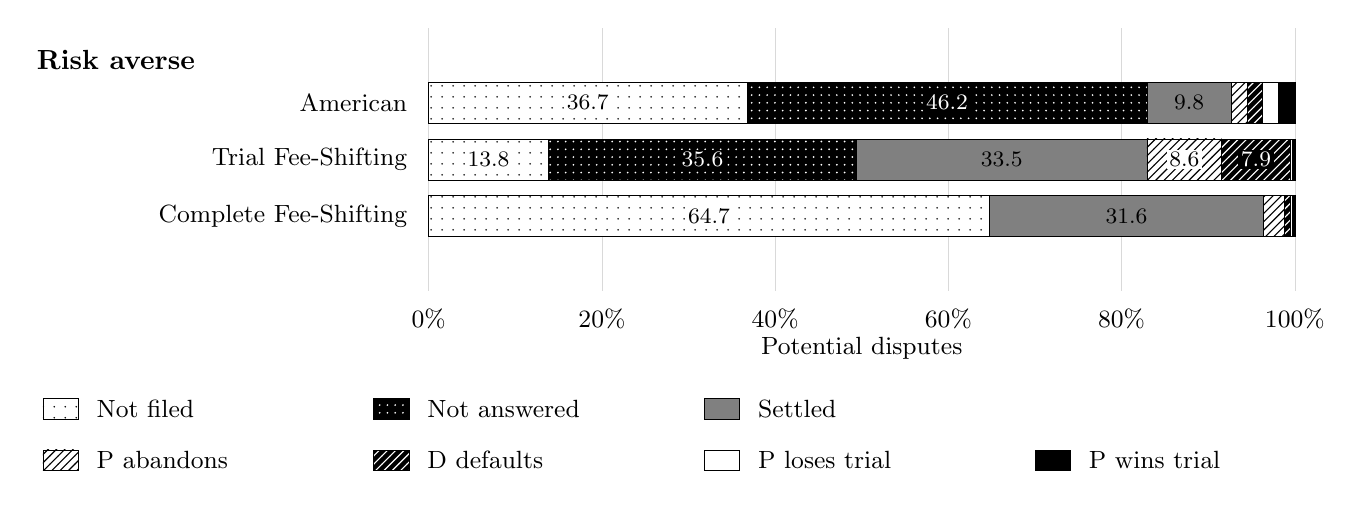
\begin{tikzpicture}[font=\small]\draw[black!15,line width=.2pt] (5.1,.65) -- (5.1,3.99);
\node[anchor=north] at (5.1,.55) {0\%};
\draw[black!15,line width=.2pt] (7.3,.65) -- (7.3,3.99);
\node[anchor=north] at (7.3,.55) {20\%};
\draw[black!15,line width=.2pt] (9.5,.65) -- (9.5,3.99);
\node[anchor=north] at (9.5,.55) {40\%};
\draw[black!15,line width=.2pt] (11.7,.65) -- (11.7,3.99);
\node[anchor=north] at (11.7,.55) {60\%};
\draw[black!15,line width=.2pt] (13.9,.65) -- (13.9,3.99);
\node[anchor=north] at (13.9,.55) {80\%};
\draw[black!15,line width=.2pt] (16.1,.65) -- (16.1,3.99);
\node[anchor=north] at (16.1,.55) {100\%};
\node[anchor=west,font=\bfseries] at (0,3.59) {\mbox{Risk} \mbox{averse}};
\node[anchor=east] at (4.95,3.04) {American};
\path[preaction={fill=white,draw=none},pattern={Dots[distance=4pt,radius=.35pt]},pattern color=black,draw=black,line width=.25pt] (5.1,2.78) rectangle (9.14206,3.3);
\node[text=black,fill=white,font=\footnotesize,inner sep=1pt] at (7.12103,3.04) {36.7};
\path[preaction={fill=black,draw=none},pattern={Dots[distance=2.8pt,radius=.35pt]},pattern color=white,draw=black,line width=.25pt] (9.14206,2.78) rectangle (14.222421,3.3);
\node[text=white,fill=black,font=\footnotesize,inner sep=1pt] at (11.682241,3.04) {46.2};
\path[fill=black!50,draw=black,line width=.25pt] (14.222421,2.78) rectangle (15.295049,3.3);
\node[text=black,fill=none,font=\footnotesize,inner sep=1pt] at (14.758735,3.04) {9.8};
\path[preaction={fill=white,draw=none},pattern={north east lines},pattern color=black,draw=black,line width=.25pt] (15.295049,2.78) rectangle (15.496712,3.3);
\path[preaction={fill=black,draw=none},pattern={north east lines},pattern color=white,draw=black,line width=.25pt] (15.496712,2.78) rectangle (15.692213,3.3);
\path[fill=white,draw=black,line width=.25pt] (15.692213,2.78) rectangle (15.892624,3.3);
\path[fill=black,draw=black,line width=.25pt] (15.892624,2.78) rectangle (16.099998,3.3);
\node[anchor=east] at (4.95,2.32) {Trial Fee-Shifting};
\path[preaction={fill=white,draw=none},pattern={Dots[distance=4pt,radius=.35pt]},pattern color=black,draw=black,line width=.25pt] (5.1,2.06) rectangle (6.62141,2.58);
\node[text=black,fill=white,font=\footnotesize,inner sep=1pt] at (5.860705,2.32) {13.8};
\path[preaction={fill=black,draw=none},pattern={Dots[distance=2.8pt,radius=.35pt]},pattern color=white,draw=black,line width=.25pt] (6.62141,2.06) rectangle (10.532119,2.58);
\node[text=white,fill=black,font=\footnotesize,inner sep=1pt] at (8.576765,2.32) {35.6};
\path[fill=black!50,draw=black,line width=.25pt] (10.532119,2.06) rectangle (14.221662,2.58);
\node[text=black,fill=none,font=\footnotesize,inner sep=1pt] at (12.376891,2.32) {33.5};
\path[preaction={fill=white,draw=none},pattern={north east lines},pattern color=black,draw=black,line width=.25pt] (14.221662,2.06) rectangle (15.172279,2.58);
\node[text=black,fill=white,font=\footnotesize,inner sep=1pt] at (14.69697,2.32) {8.6};
\path[preaction={fill=black,draw=none},pattern={north east lines},pattern color=white,draw=black,line width=.25pt] (15.172279,2.06) rectangle (16.041614,2.58);
\node[text=white,fill=black,font=\footnotesize,inner sep=1pt] at (15.606946,2.32) {7.9};
\path[fill=white,draw=black,line width=.25pt] (16.041614,2.06) rectangle (16.074285,2.58);
\path[fill=black,draw=black,line width=.25pt] (16.074285,2.06) rectangle (16.100005,2.58);
\node[anchor=east] at (4.95,1.6) {Complete Fee-Shifting};
\path[preaction={fill=white,draw=none},pattern={Dots[distance=4pt,radius=.35pt]},pattern color=black,draw=black,line width=.25pt] (5.1,1.34) rectangle (12.222148,1.86);
\node[text=black,fill=white,font=\footnotesize,inner sep=1pt] at (8.661074,1.6) {64.7};
\path[fill=black!50,draw=black,line width=.25pt] (12.222148,1.34) rectangle (15.70103,1.86);
\node[text=black,fill=none,font=\footnotesize,inner sep=1pt] at (13.961589,1.6) {31.6};
\path[preaction={fill=white,draw=none},pattern={north east lines},pattern color=black,draw=black,line width=.25pt] (15.70103,1.34) rectangle (15.964591,1.86);
\path[preaction={fill=black,draw=none},pattern={north east lines},pattern color=white,draw=black,line width=.25pt] (15.964591,1.34) rectangle (16.04737,1.86);
\path[fill=white,draw=black,line width=.25pt] (16.04737,1.34) rectangle (16.063696,1.86);
\path[fill=black,draw=black,line width=.25pt] (16.063696,1.34) rectangle (16.099998,1.86);
\node at (10.6,-.08) {Potential disputes};
\path[preaction={fill=white,draw=none},pattern={Dots[distance=4pt,radius=.35pt]},pattern color=black,draw=black,line width=.25pt] (0.2,-0.98) rectangle (0.65,-0.72);
\node[anchor=west] at (0.76,-0.85) {Not filed};
\path[preaction={fill=black,draw=none},pattern={Dots[distance=2.8pt,radius=.35pt]},pattern color=white,draw=black,line width=.25pt] (4.4,-0.98) rectangle (4.85,-0.72);
\node[anchor=west] at (4.96,-0.85) {Not answered};
\path[fill=black!50,draw=black,line width=.25pt] (8.6,-0.98) rectangle (9.05,-0.72);
\node[anchor=west] at (9.16,-0.85) {Settled};
\path[preaction={fill=white,draw=none},pattern={north east lines},pattern color=black,draw=black,line width=.25pt] (0.2,-1.63) rectangle (0.65,-1.37);
\node[anchor=west] at (0.76,-1.5) {P abandons};
\path[preaction={fill=black,draw=none},pattern={north east lines},pattern color=white,draw=black,line width=.25pt] (4.4,-1.63) rectangle (4.85,-1.37);
\node[anchor=west] at (4.96,-1.5) {D defaults};
\path[fill=white,draw=black,line width=.25pt] (8.6,-1.63) rectangle (9.05,-1.37);
\node[anchor=west] at (9.16,-1.5) {P loses trial};
\path[fill=black,draw=black,line width=.25pt] (12.8,-1.63) rectangle (13.25,-1.37);
\node[anchor=west] at (13.36,-1.5) {P wins trial};
\end{tikzpicture}
\end{document}
